\documentclass[tikz,class=minimal,border=0pt]{standalone}

\usetikzlibrary{shapes,arrows}

\usepackage{booktabs}
\usepackage{multirow}
\usepackage{amsmath}
\usepackage{color}

\usepackage{fontspec}
\setmainfont{Arial}

\definecolor{fillcolour}{HTML}{89d0F5}

\usepackage{tabto}

\begin{document}

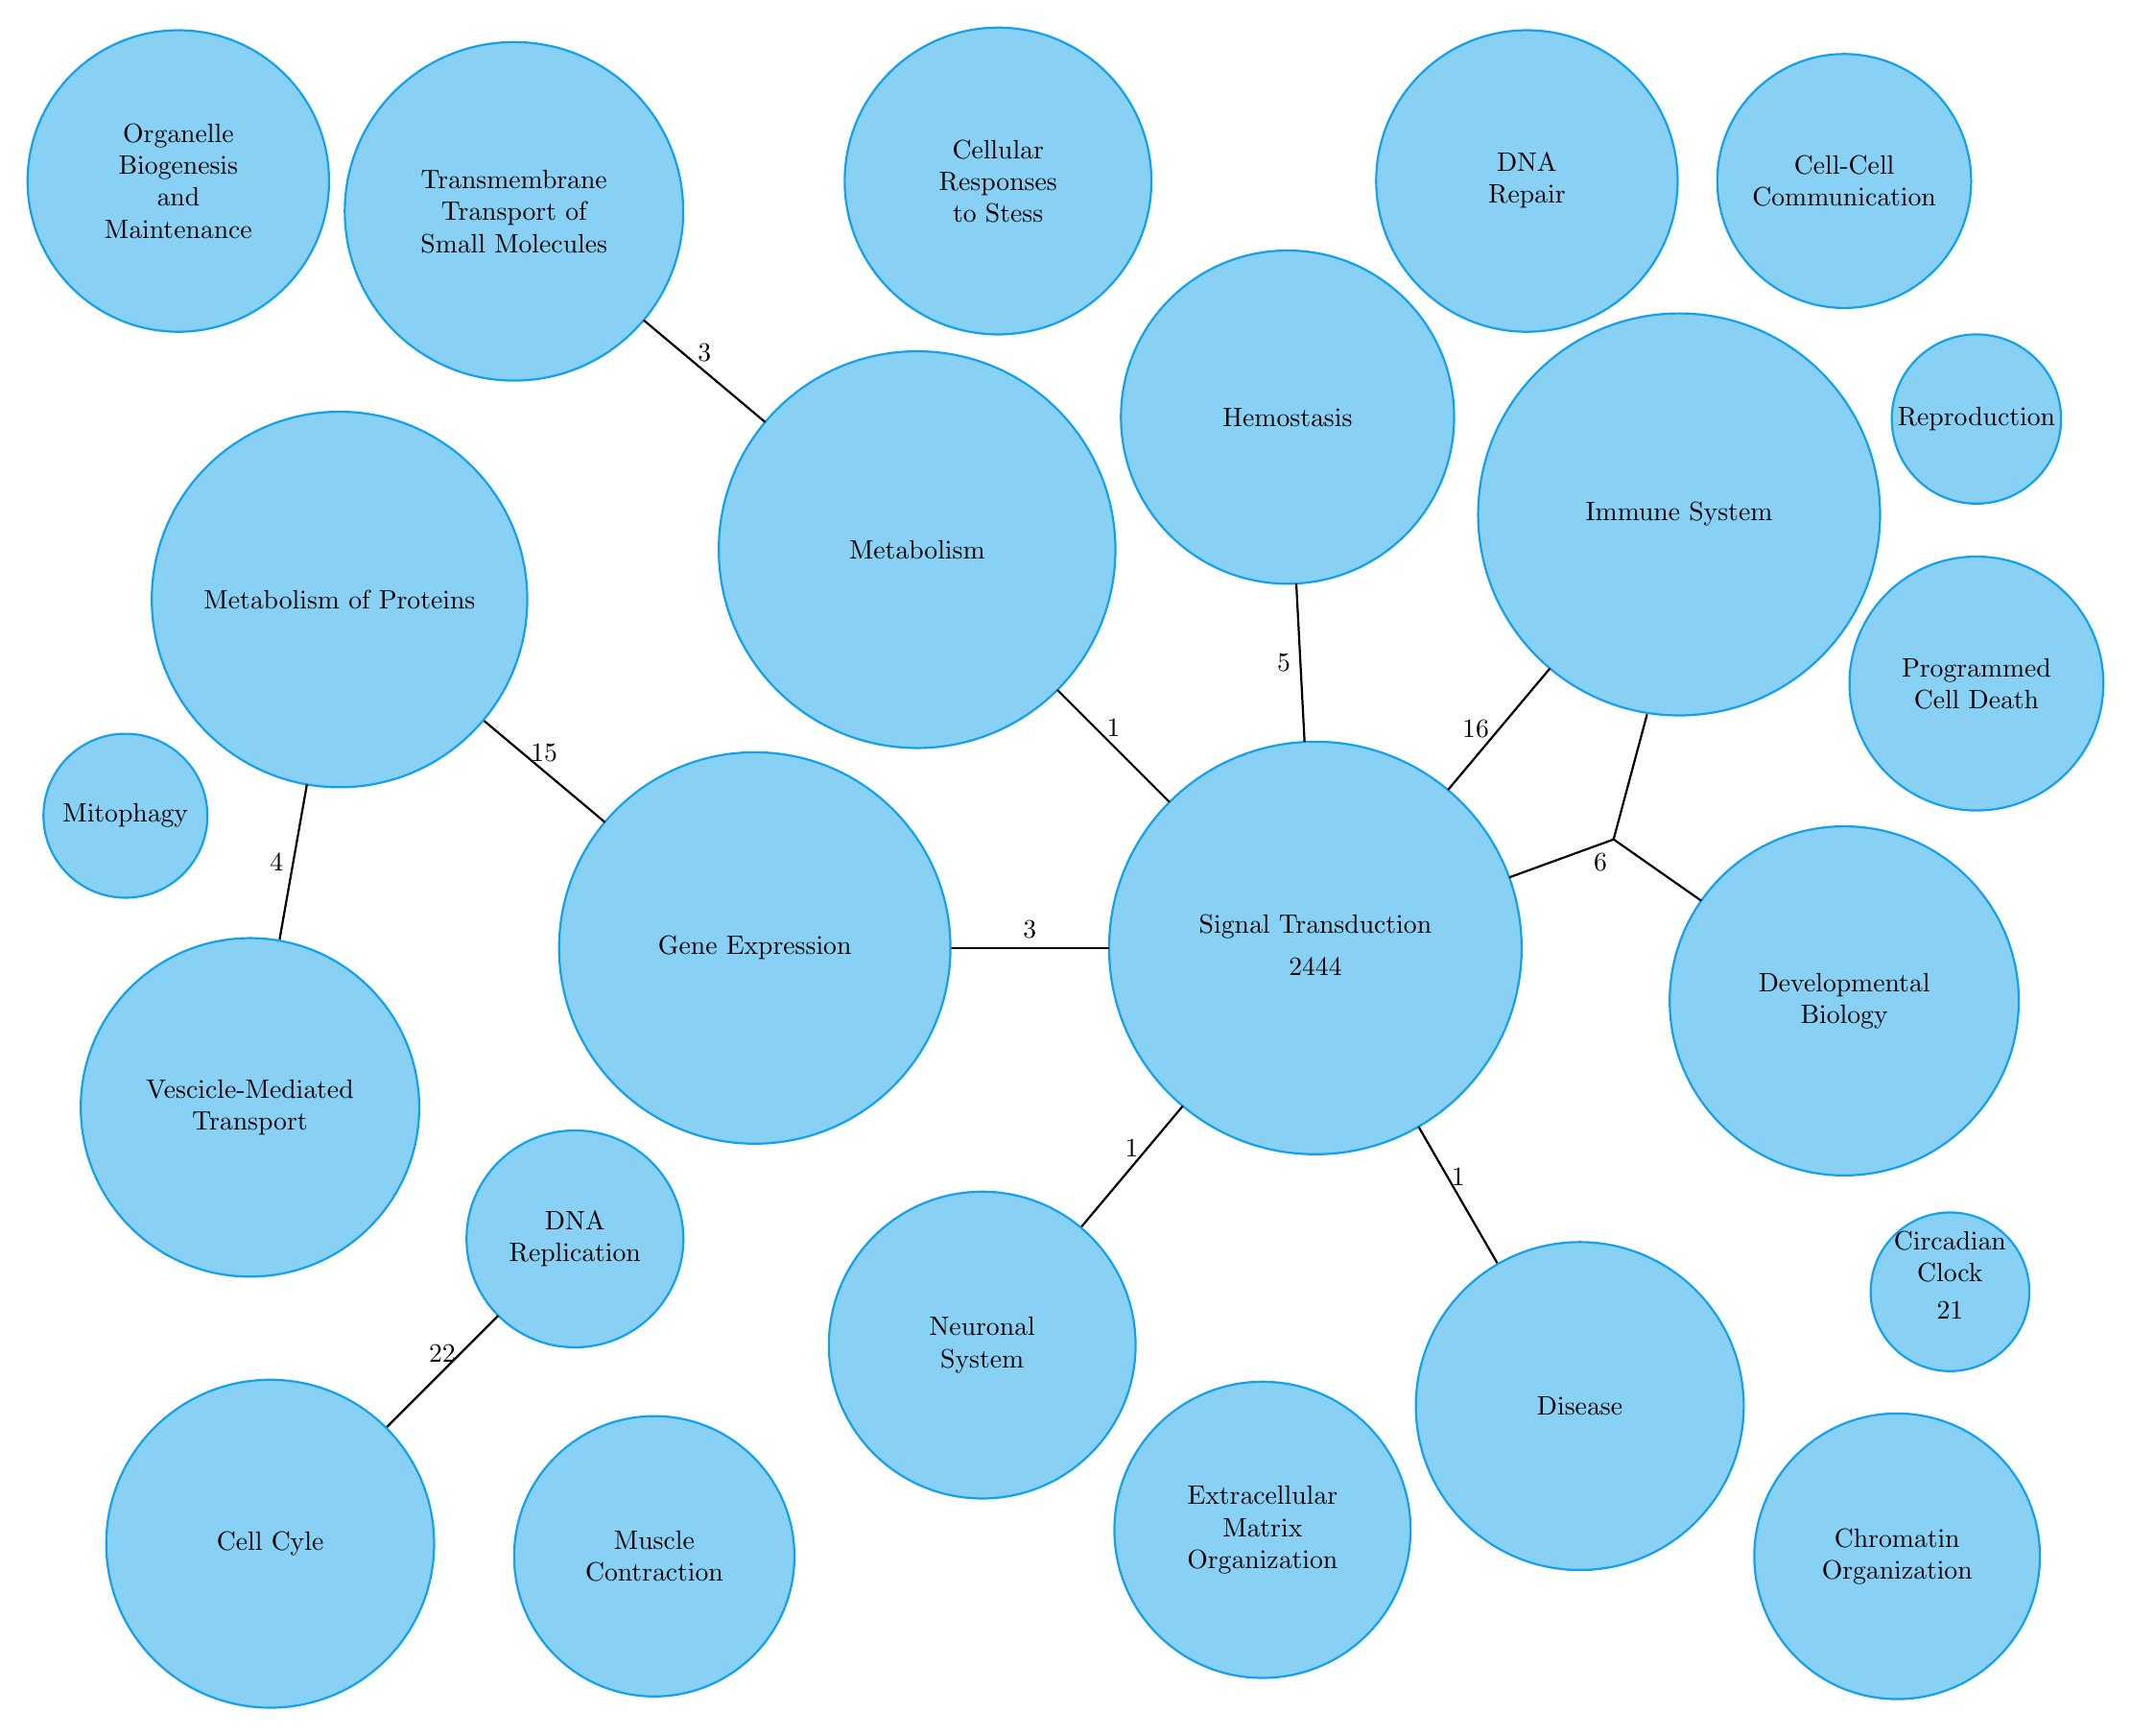
\begin{tikzpicture}[scale=0.35]
% Signal Transduction
\draw[fillcolour!200,fill=fillcolour,thick] (0,5) circle (7.8) node[anchor=south, color=black] {Signal Transduction} node[anchor=north, color=black] {2444};
% Connect Signal Transduction to Immune System
\draw[fillcolour!200,fill=fillcolour,thick] (0,5) ++(50:7.8) ++(50:6) ++(50:7.6) circle (7.6) node[color=black] {Immune System};
\draw[black,thick] (0,5) ++(50:7.8) -- ++(50:6) node[midway,left] {16};
% Connect Signal Transduction to Hemostasis
\draw[fillcolour!200,fill=fillcolour,thick] (0,5) ++(93:7.8) ++(93:6) ++(93:6.3) circle (6.3) node[color=black] {Hemostasis};
\draw[black,thick] (0,5) ++(93:7.8) -- ++(93:6) node[midway,left] {5};
% Connect Signal Transduction to Metabolism
\draw[fillcolour!200,fill=fillcolour,thick] (0,5) ++(135:7.8) ++(135:6) ++(135:7.5) circle (7.5) node[color=black] {Metabolism};
\draw[black,thick] (0,5) ++(135:7.8) -- ++(135:6) node[midway,above] {1};
%% Connect Metabolism to Transmembrane Transport of Small Molecules
\draw[fillcolour!200,fill=fillcolour,thick] (0,5) ++(135:7.8) ++(135:6) ++(135:7.5) ++(140:7.5) ++(140:6) ++(140:6.4) circle (6.4) node[color=black, align=center] {Transmembrane\\Transport of\\Small Molecules};
\draw[black,thick] (0,5) ++(135:7.8) ++(135:6) ++(135:7.5) ++(140:7.5) -- ++(140:6) node[midway,above] {3};
% Connect Signal Transduction to Gene Expression
\draw[black,thick] (0,5) ++(180:7.8) -- ++(180:6) node[midway,above] {3};
\draw[fillcolour!200,fill=fillcolour,thick] (0,5) ++(180:7.8) ++(180:6) ++(180:7.4) [fillcolour!200,fill=fillcolour] circle (7.4) node[color=black] {Gene Expression};
%% Connect Gene Expression to Metabolism of Proteins
\draw[black,thick] (0,5) ++(180:7.8) ++(180:6) ++(180:7.4) ++(140:7.4) -- ++(140:6) node[midway,above] {15};
\draw[fillcolour!200,fill=fillcolour,thick] (0,5) ++(180:7.8) ++(180:6) ++(180:7.4) ++(140:7.4) ++(140:6) ++(140:7.1) circle (7.1) node[color=black] {Metabolism of Proteins};
%% Connect Metabolism of Proteins to Vesicle-Mediated Transport
\draw[black,thick] (0,5) ++(180:7.8) ++(180:6) ++(180:7.4) ++(140:7.4) ++(140:6) ++(140:7.1) ++(260:7.1) -- ++(260:6) node[midway,left, ] {4};
\draw[fillcolour!200,fill=fillcolour,thick] (0,5) ++(180:7.8) ++(180:6) ++(180:7.4) ++(140:7.4) ++(140:6) ++(140:7.1) ++(260:7.1) ++(260:6) ++(260:6.4) circle (6.4) node[color=black, align=center] {Vescicle-Mediated\\Transport};
% Connect Signal Transduction to Disease
\draw[black,thick] (0,5) ++(300:7.8) -- ++(300:6) node[midway,above] {1};
\draw[fillcolour!200,fill=fillcolour,thick] (0,5) ++(300:7.8) ++(300:6) ++(300:6.2) circle (6.2) node[color=black] {Disease};
% Connect Signal Transduction to Neuronal System
\draw[black,thick] (0,5) ++(230:7.8) -- ++(230:6) node[midway,above] {1};
\draw[fillcolour!200,fill=fillcolour,thick] (0,5) ++(230:7.8) ++(230:6) ++(230:5.8) circle (5.8) node[color=black, align=center] {Neuronal\\System};

% Connect DNA Recplication to Cell Cycle
\draw[fillcolour!200,fill=fillcolour,thick] (-28,-6) circle (4.1) node[color=black,align=center] {DNA\\Replication};
\draw[black,thick] (-28,-6) ++(225:4.1) -- ++(225:6) node[midway,above] {22};
\draw[fillcolour!200,fill=fillcolour,thick] (-28,-6) ++(225:4.1) ++(225:6) ++(225:6.2) circle (6.2) node[color=black] {Cell Cyle};

% Developmental Biology
\draw[fillcolour!200,fill=fillcolour,thick] (20,3) circle (6.6) node[color=black,align=center] {Developmental\\Biology};
\draw[black,thick] ( 0,5) ++( 20: 7.8) -- +( 20:4.2) node[very near end,below] {6};
\draw[black,thick] (20,3) ++(145: 6.6) -- +(145:4.1);
\draw[black,thick] ( 0,5) ++( 20:12  ) -- +( 75:4.9);


% DNA Repair
\draw[fillcolour!200,fill=fillcolour,thick] (8,34) circle (5.7) node[color=black,align=center] {DNA\\Repair};

% Cellular Responses to Stress
\draw[fillcolour!200,fill=fillcolour,thick] (-12,34) circle (5.8) node[color=black,align=center] {Cellular\\Responses\\to Stess};

% Organelle Biogenesis and Maintenance
\draw[fillcolour!200,fill=fillcolour,thick] (-43,34) circle (5.7) node[color=black,align=center] {Organelle\\Biogenesis\\and\\Maintenance};

% Extracellular Matrix Organization
\draw[fillcolour!200,fill=fillcolour,thick] (-2,-17) circle (5.6) node[color=black,align=center] {Extracellular\\Matrix\\Organization};

% Chromatin Organization
\draw[fillcolour!200,fill=fillcolour,thick] (22,-18) circle (5.4) node[color=black,align=center] {Chromatin\\Organization};

% Muscle Contraction
\draw[fillcolour!200,fill=fillcolour,thick] (-25,-18) circle (5.3) node[color=black,align=center] {Muscle\\Contraction};

% Circadian Clock
\draw[fillcolour!200,fill=fillcolour,thick] (24,-8) circle (3) node[anchor=south,color=black,align=center] {Circadian\\Clock} node[anchor=north, color=black] {21};

% Cell-Cell communication
\draw[fillcolour!200,fill=fillcolour,thick] (20,34) circle (4.8) node[color=black,align=center] {Cell-Cell\\Communication};

% Programemd Cell Death
\draw[fillcolour!200,fill=fillcolour,thick] (25,15) circle (4.8) node[color=black,align=center] {Programmed\\Cell Death};

% Reproduction
\draw[fillcolour!200,fill=fillcolour,thick] (25,25) circle (3.2) node[color=black,align=center,color=black] {Reproduction};

% Mitphagy
\draw[fillcolour!200,fill=fillcolour,thick] (-45,10) circle (3.1) node[color=black,align=center] {Mitophagy};

\end{tikzpicture}
\end{document}